\section{System's perspective}
\subsection{Design}
When faced with the initial task of refactoring the MiniTwit system, we agreed to choose a stack consisting of technologies at least one member of the group had experience with.
This enabled us to both have the advantage of working with something familiar and gave the opportunity to learn something new. 

We chose React with Typescript for the frontend and when making the MiniTwit application we prioritized having the same functionality as the existing Flask application. As a result of this, the page setup and styling is identical to the original application.
We have used C\# for our backend. The data access technology used is Entity Framework Core.\\

Our Database is a Managed Azure SQL database hosted on Azure. Originally we had Azure SQL Edge running in Docker but as the database data is important to save persistently we switched to Azure SQL running on a Microsoft Azure server. Azure allowed us to enable automatic tuning of the different tables that improved performance drastically (Indexation of tables). More on these topics in future sections.

\subsection{Architecture}
This sections aims to describe the architecture of our system using Christensens 3+1 model \cite{architecturemodel} by showing:
\begin{itemize}
    \item Requirements
    \item Module viewpoint 
    \item Component \& connectors viewpoint 
    \item Allocation / deployment viewpoint
\end{itemize}

The system is separated into a three-tier architecture which is shown in Figure \ref{fig:Threetier}.
The diagram includes the course simulator (which is not in our control) as a component as it has a significant impact on the system.
\begin{figure}[H]
 \centering
 \includegraphics[width = 0.4\textwidth]{images/three\_tier.png}
 \caption{Overall architecture}
 \label{fig:Threetier}
\end{figure}

\subsubsection{Requirements}    
This section concerns the "+1" part of the 3+1 model i.e. the architectural requirements. \\
Though they referenced as "scenario-based" and "quality attribute-based" in the literature, this 
report will use the terms functional and non-functional requirements respectively. \\

\noindent
\textbf{Functional requirements}
\begin{enumerate}
    \item The system must provide the same functionality as the original MiniTwit system given at the introduction of the course
    \item The system must expose an API which adheres to the requirements of \cite{apispec} 
\end{enumerate} 

\noindent
\textbf{Non-functional requirements}
\begin{enumerate}
    \item The systems backend must be written in C\# 
    \item The systems frontend must be written in React with Typescript
    \item The system must be containerized with Docker ensuring isolation and portability
    \item The system must be deployed on DigitalOcean
    \item The system must be performant, scaleable and reliable in accordance to the SLA, Appendix \ref{app:SLA}.
\end{enumerate}
    
\subsubsection{Module viewpoint}
At the highest level, the system is divided into backend and frontend.\\

The following package diagram gives a high-level overview of the backend's file structure and dependencies.
\begin{figure}[H]
 \centering
 \includegraphics[width = 0.4\textwidth]{images/backend\_package\_overview.png}
 \caption{Backend Package overview showing how data is accessed in the system.}
 \label{fig:BackendPackageDiagram}
\end{figure}
\begin{itemize}
    \item \textbf{Domain:} contains the business entities of the system i.e. model and DTO classes representing users, tweets and followers.
    \item \textbf{DataAccess:} contains the class that handles sessions and communication with the database.
    \item \textbf{MiniTwitAPI:} houses the controller classes that make up both the public and internal APIs of the system, which are two separate units. 
\end{itemize}
A complete package diagram for the backend, including all relevant artifacts, etc., can be seen in figure \ref{fig:BackendCompletePackageDiagram}. \\

\begin{figure}[H]
 \centering
 \includegraphics[width = 0.5\textwidth]{images/backend\_complete\_package.png}
 \caption{Package diagram showing our backend artifacts, dependencies omitted for clarity}
 \label{fig:BackendCompletePackageDiagram}
\end{figure}

\newpage
The next part of the program is the frontend, of which a package diagram is shown in figure \ref{fig:FrontendPackageDiagram}.
Only the "src" package contains files of interest i.e. that we have written, as opposed to configuration or boilerplate files and as such the contents of "public", "nginx" and the root folder is not shown in the diagram. The artifacts represent the individual pages of the website as well as subcomponents, media, stylesheets and some configuration-files that are React-specific. The naming of the pages reflects the naming from the original page structure provided.

\begin{figure}[H]
 \centering
 \includegraphics[width = \textwidth]{images/package\_frontend.png}
 \caption{Package diagram of the frontend folder, some folders omitted for clarity}
 \label{fig:FrontendPackageDiagram}
\end{figure}


\subsubsection{Components \& connectors viewpoint}
Figure \ref{fig:CompleteComponentDiagram} shows the six components e.g. Docker containers of our primary DigitalOcean droplet and how they interact with each other at runtime. In the diagram, the "MiniTwit backend" component contains two separate API subcomponents. The actual Docker container uses the same port to handle both API requests from the simulator and from the website but we have chosen to show it as two components here to indicate that they serve two different purposes.
\begin{figure}[H]
 \centering
 \includegraphics[width = \textwidth]{images/all\_components.png}
 \caption{Component diagram of our primary DigitalOcean droplet, Docker volumes omitted}
 \label{fig:CompleteComponentDiagram}
\end{figure}
\subsubsection{Allocation / deployment viewpoint}
As seen in Figure \ref{fig:DeploymentDiagram}, the system consists of a managed database on Microsoft's Azure platform as well as two separate droplets on DigitalOcean. The two droplets constitute our scaling setup which is described in depth in a future section. \\
% The most interesting parts to examine more deeply (from an architectural perspective) is the Docker containers for frontend and backend, as we wrote the code for those parts whereas the remaining 4 Docker containers (on the minitwit droplet) are just third party dependencies. \\ 
\begin{figure}[H]
 \centering
 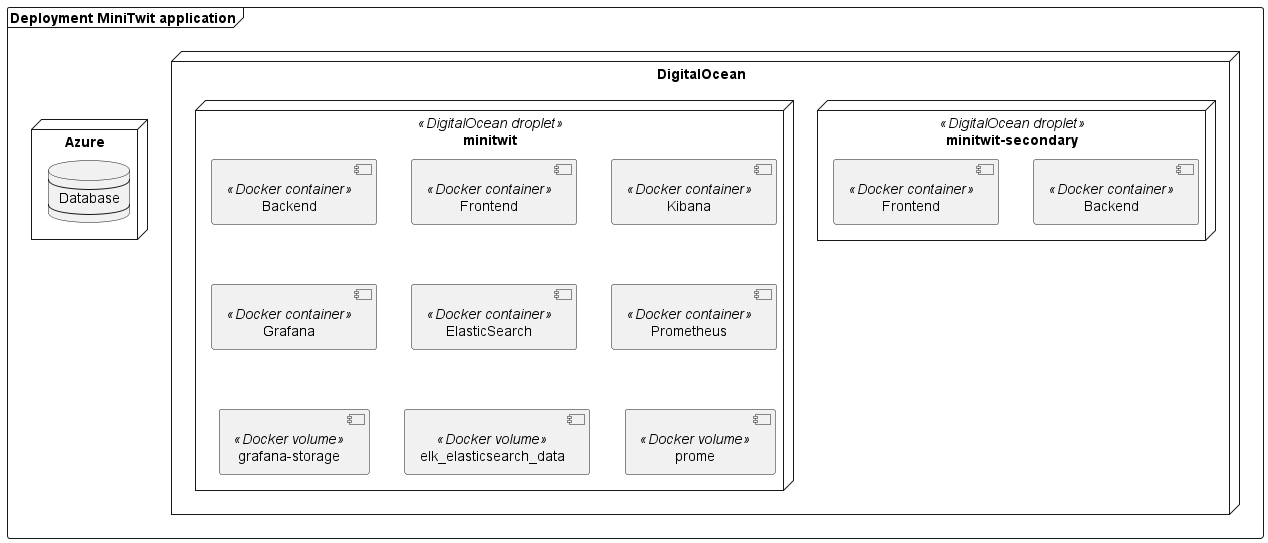
\includegraphics[width = \textwidth]{images/deployment.png}
 \caption{Deployment diagram illustrating the overall deployment view of our MiniTwit system including Docker volumes for monitoring and logging}
 \label{fig:DeploymentDiagram}
\end{figure}
\noindent
Both droplets are hosted on servers located in Frankfurt, Germany and have the following specs \\
\begin{table}[H]
\centering
\begin{tabular}{|l|l|l|l} 
\cline{1-3}
           & Primary & Secondary &   \\ 
\cline{1-3}
vCPU       & 1       & 1         &   \\ 
\cline{1-3}
Memory     & 2 GB    & 1 GB      &   \\ 
\cline{1-3}
Disc Space & 50 GB   & 25 GB     &   \\
\cline{1-3}
\end{tabular}
\end{table}

\noindent
They do not have the same specifications as they do not handle the same tasks but this will be elaborated in a later section.

\subsection{Dependencies - technologies and tools}
The following is a table of the dependencies and tools that the project relies on as well as a brief comment on what they're used for.
\begin{center}
\begin{tabularx}{\textwidth}{|X|l|}
 \hline
 \textbf{Name} & \textbf{Responsibility}  \\ [0.5ex] 
 \hline\hline
 \textbf{Git} & Version control  \\ 
 \hline
 \textbf{GitHub} & Repository management \\
 \hline
 \textbf{C\# / ASP.NET CORE / .NET} & Used for our backend \\
 \hline
 \textbf{Typescript} & Used for React frontend \\
 \hline
 \textbf{Azure SQL Database} & The database system used for our MiniTwit application\\ 
 \hline
 \textbf{Serilog} & A library used for logging in the backend \\
 \hline
 \textbf{Prometheus} & Used for system monitoring \\
 \hline
 \textbf{Grafana} & Used to display monitoring information\\
 \hline
 \textbf{ElasticSearch} & Used to store the systems logs \\
 \hline
 \textbf{Kibana} & Used to present the aggregated logs \\
 \hline
 \textbf{Docker} & Used for containerizing the system \\
 \hline
 \textbf{Ubuntu} & The OS that our droplets run on\\
 \hline
 \textbf{React} & JavaScript library for building the website \\
 \hline
 \textbf{Nginx} & A web server that runs React\\
 \hline
 \textbf{Docker-compose} & Handling multiple docker containers \\
 \hline
 \textbf{Docker Hub} & Storing docker images \\
 \hline
 \textbf{Sonarcloud} & Static analysis \\
 \hline
 \textbf{DigitalOcean} & Provider of infrastructure \\
 \hline
 \textbf{Vagrant} & Provisioning of virtual machines \\
 \hline
 \textbf{CircleCI} & Continous integration pipeline \\
 \hline
 \textbf{Better Code Hub} & Provides static analysis of the code \\
 \hline
 \textbf{Keepalived} & High-availability / scaling \\
 \hline
 \textbf{Python} & Used in a script for switching floating IP on DigitalOcean  \\
 \hline
 \textbf{Bash} & Used as terminal for the developers and for scripts.\\
 \hline
 \textbf{SSMPT} & Used to configure the mail server.\\
 \hline
 \textbf{MailUtils} & Used to send a mail directly from a script using SSMTP server settings. \\
 \hline
 \textbf{Gmail} & Used as a central mailbox that forwards to our individual ITU mails \\[1ex] 
 \hline
\end{tabularx}
\end{center}

\subsection{Important interactions of subsystems}
The most important interactions of subsystems in our MiniTwit application are the following 
\begin{itemize}
    \item HTTP communication between frontend and backend
    \item HTTP communication between backend and the simulator
    \item HTTP communication between backend and Prometheus
    \item HTTP communication between Prometheus and Grafana
    \item HTTP communication between backend and ElasticSearch
    \item HTTP communication between ElasticSearch and Kibana
    \item Communication between the backend and the Azure database via EF Core
\end{itemize}

The sequence diagram in figure \ref{fig:SequenceDiagramPostMessage} shows the interaction between frontend, backend and database when a user posts a new message. \\
Most interactions between frontend and backend as well as between the backend and simulator follow the same flow, and as such these will not be depicted.

\begin{figure}[H]
 \centering
 \includegraphics[width = .5 \textwidth]{images/frontend\_backend\_post\_messages\_sequence.png}
 \caption{Sequence diagram depicting the interaction between frontend, backend and database when a user posts a new message}
 \label{fig:SequenceDiagramPostMessage}
\end{figure}

Figure \ref{fig:SequenceDiagramElasticBackendSim} shows an example of an interaction between the simulator, backend, ElasticSearch and database. In particular it depicts the sequence of logging and database calls that occur between a request to post a message being made and the response being returned to the simulator.

\begin{figure}[H]
 \centering
 \includegraphics[width = .9 \textwidth]{images/sim\_backend\_elastic\_sequence.png}
 \caption{Sequence diagram depicting the interactions between the simulator, our simulator API, ElasticSearch and database that happen when the simulator posts a new message from a user}
 \label{fig:SequenceDiagramElasticBackendSim}
\end{figure}

This final sequence diagram in figure \ref{fig:SequenceDiagramSimRegisterAlternative} shows the interaction between simulator, backend, database, logging and monitoring when a user is created, including the two possible execution paths determined by whether the user already exists or not.
Note that Kibana and Grafana will regularly retrieve data from ElasticSearch and Prometheus respectively but these interactions have been omitted along with any responses that ElasticSearch and Prometheus might give. 
\begin{figure}[H]
 \centering
 \includegraphics[width = \textwidth]{images/sim\_register\_user_alternative.png}
 \caption{Sequence diagram depicting the interactions between the simulator, our simulator API, ElasticSearch and database that happen when the simulator posts a new message from a user}
 \label{fig:SequenceDiagramSimRegisterAlternative}
\end{figure}

\subsection{Current state of the system}
The current system has an improved availability with the use of Keepalived. The system is easier to maintain, because the system now uses static analysis and diagrams that makes the development of the system more smooth. 
Results from the static analysis tool bettercodehub.com can be seen in Appendix \ref{app:bettercodehub}.
Containerization of the system creates a uniform and isolated development environment. 
Moreover, a database abstraction layer reduces vendor-specific coupling and improves the systems security against e.g. SQL injection.  
The system uses continues integration pipelines to increase the reliability, as well as continuous delivery that optimises the deployment of the system for the developers. The system has monitoring and logging providing insights into the running system.  
\\
The following are features and technologies that we would have liked to implement but did not.

\begin{enumerate}
    \item Automatic release on deployment
    \item Running tests as part of CI (and terminating on test failure)
    \item Rolling updates (and including secondary server in CI)
    \item Provisioning of VM for secondary server
    \item Infrastructure as code with Terraform
\end{enumerate}

\subsection{License compatibility}
The license chosen for this project is: \textbf{GNU GPL-3.0}. A list of the licenses for direct dependencies in the project can be seen in appendix \ref{ssec:licences}. According to Wheeler\cite{LicenseComp} the projects licence is compatible with the following licenses: 
\begin{itemize}
    \item MIT
    \item Apache 2.0
    \item GNU GPL-3.0
    \item AGPL v2 
\end{itemize}
The license of the project should therefore be compatible with the licenses of its direct dependencies.